\documentclass[dvipsnames, svgnames, x11names]{beamer}
\usetheme{mytheme}


\title{第六章}
\subtitle{电化学}
\author{张斌}
\institute[理工系]{河北农业大学 理工系}
\date{\the\year 年 \the\month 月}


\begin{document}

	\begin{frame}
		\titlepage
		\thispagestyle{empty}
		\addtocounter{framenumber}{-1}
	\end{frame}

	\begin{frame}{}
        \begin{center}
            {\Huge \cbf{目 \ 录}}
        \end{center}
		\tableofcontents
		\thispagestyle{empty}
		\addtocounter{framenumber}{-1}
	\end{frame}




	\section{可逆电池}


	\begin{frame}
		\frametitle{电池}
	
		\begin{minipage}{0.48\linewidth}
			\begin{itemize}
				\item 一般化学反应体系的能量大部分是以热的形式与环境进行交换，而不做功。
				\item 在氧化还原反应中，电子从还原剂转移到氧化剂，如果在适当的装置中进行反应，能够产生电流用以做功。
				\item 这种装置称为原电池
				\item 原电池将化学能转化为电能的过程称为放电。
			\end{itemize}
		\end{minipage}\hfill
		\begin{minipage}{0.48\linewidth}
			
\includegraphics[width=\linewidth]{figures/fig6.1.png}
		\end{minipage}
	
	\end{frame}
	
	
	\begin{frame}
		\frametitle{可逆电池}
	
		可逆电池须具备以下条件：
		\begin{itemize}
			\item 电池在充、放电时发生的反应须互为可逆反应。（化学反应可逆）
			\item 电池充放电时的能量转换必须可逆，即通过电池的电流无限小，无热功转化。（能量转化可逆）
		\end{itemize}
		\begin{minipage}{0.3\linewidth}
			\begin{figure}
				\centering
				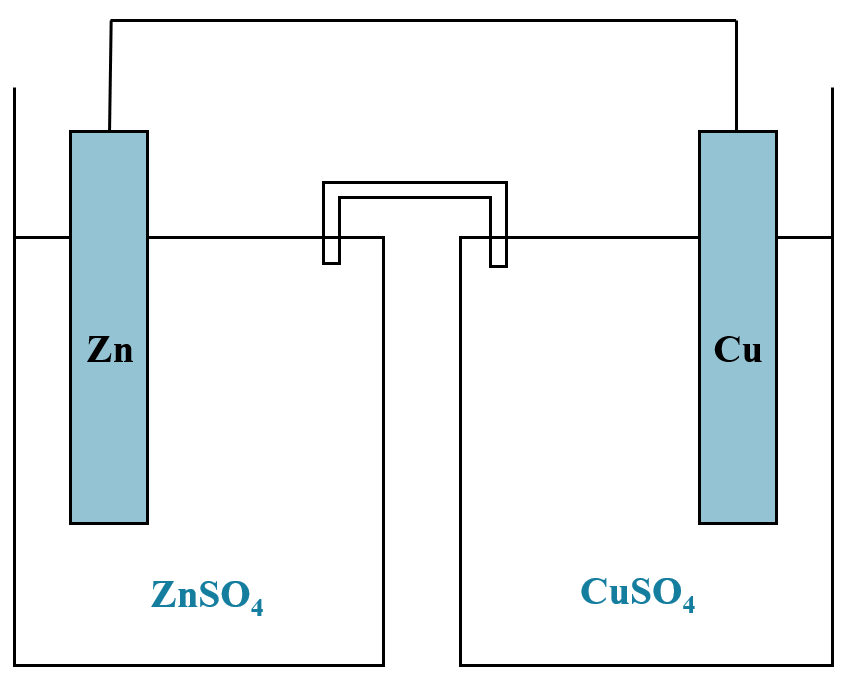
\includegraphics[width=\linewidth]{figures/fig6.1a.png}
			\end{figure}        
		\end{minipage}\hfill
		\begin{minipage}{0.08\linewidth}
				~~放电
	
				~~
	
				~~
	
				~~充电
		\end{minipage}\hfill
		\begin{minipage}{0.6\linewidth}
			\begin{itemize}
				\item[阳] \ch{Zn - 2 e- -> Zn^{2+}}
				\item[阴] \ch{Cu^{2+} + 2 e- -> Cu}
				\item[总] \ch{Zn(s) + Cu^{2+} -> Zn^{2+} + Cu(s)}
			\end{itemize}
			
			\begin{itemize}
				\item[$(-)$] \ch{Zn^{2+} + 2 e- -> Zn}
				\item[$(+)$] \ch{Cu - 2 e- -> Cu^{2+}}
				\item[总] \ch{Zn^{2+} + Cu(s) -> Zn(s) + Cu^{2+}}
			\end{itemize}
		\end{minipage}
	
	\end{frame}
	
	
	\begin{frame}
		\frametitle{不可逆电池}
	
		在电池充电和放电时，电池反应不是可逆反应，或工作电流较大，有热功转换，电池就不是可逆电池。
	
		\begin{minipage}{0.3\linewidth}
			\begin{figure}
				\centering
				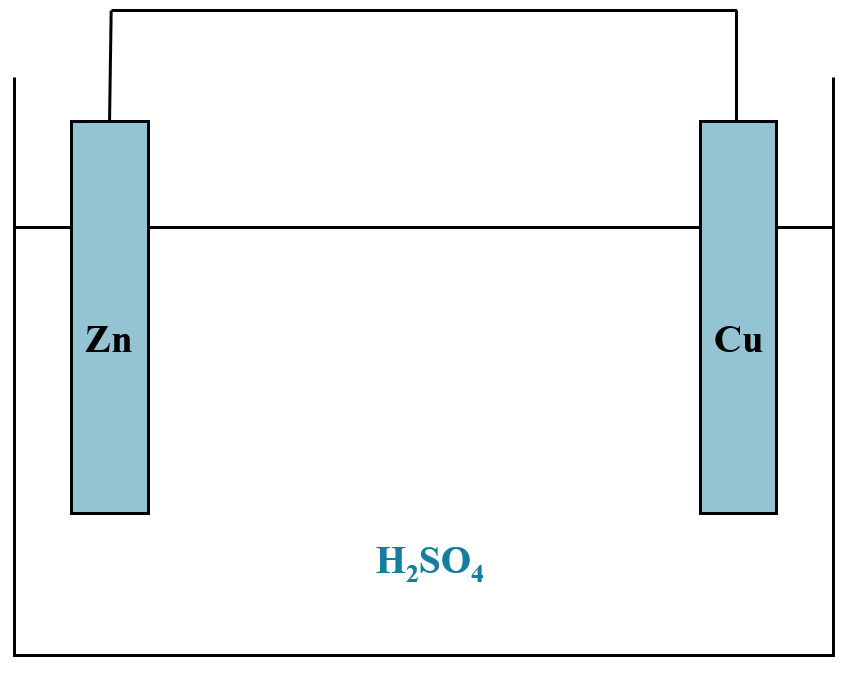
\includegraphics[width=\linewidth]{figures/fig6.1b.png}
			\end{figure}        
		\end{minipage}\hfill
		\begin{minipage}{0.08\linewidth}
				~~放电
	
				~~
	
				~~
	
				~~充电
		\end{minipage}\hfill
		\begin{minipage}{0.6\linewidth}
			\begin{itemize}
				\item[阳] \ch{Zn - 2 e- -> Zn^{2+}}
				\item[阴] \ch{2 H+ + 2 e- -> H2 (g)}
				\item[总] \ch{2 H+ + Zn -> Zn^{2+} + H2 (g)}
			\end{itemize}
			
			\begin{itemize}
				\item[$(-)$] \ch{2 H+ + 2 e- -> H2 (g)}
				\item[$(+)$] \ch{Cu - 2 e- -> Cu^{2+}}
				\item[总] \ch{2 H+ + Cu -> Cu^{2+} + H2 (g)}
			\end{itemize}
		\end{minipage}
	
	\end{frame}
	
	
	\begin{frame}
		\frametitle{可逆电极的类型和电极反应}
	
		\begin{itemize}
			\item[1.] \cbf{金属电极} 
		\end{itemize}
		由金属浸在含有该金属离子的溶液中构成。
		\begin{itemize}
			\item \bf{Zn电极 }
			
				作为正极时 \qquad \ch{ZnSO4(aq) \ |\  Zn(s)} \qquad \ch{Zn^{2+} + 2 e- -> Zn(s)}
	
				作为负极时 \qquad \ch{Zn(s) \ |\  ZnSO4(aq)} \qquad \ch{Zn(s) - 2 e- -> Zn^{2+}}
			\item \bf{汞齐电极 }
			
			作正极时 \quad \ch{Na+ (a_{Na+}) \ |\  Na(Hg)(a)} \quad \ch{Na+ (a_{Na+}) + Hg(l) + e- -> Na(Hg)(a)}
	
			作负极时 \quad \ch{Na(Hg)(a) \ |\  Na+ (a_{Na+})} \quad \ch{Na(Hg)(a) - e- -> Na+ (a_{Na+}) + Hg(l)}
		\end{itemize}
	
	\end{frame}
	
	
	\begin{frame}
		\frametitle{可逆电极的类型和电极反应}
	
		\begin{itemize}
			\item[2.] \cbf{气体电极} 
		\end{itemize}
		由惰性金属（通常用Pt或Au为导电体）插入某气体及其离子溶液中构成的电极。
		\begin{itemize}
			\item \bf{氢电极 }
			
			$\mathrm{H^+}(\mathrm{a_{H^+}})$\ch{ \ |\  H2 (g) \ |\  Pt(s)} \qquad $2\mathrm{H}^+(\mathrm{a_{H^+}})$ \ch{+ 2 e- -> H2 (g)}
	
			$\mathrm{OH^-}(\mathrm{a_{OH^-}})$\ch{ \ |\  H2 (g) \ |\  Pt(s)} \qquad \ch{2 H2O + 2 e- -> H2 (g) +} $2\mathrm{OH}^-(\mathrm{a_{OH^-}})$
			\item \bf{氧电极 }
			
			$\mathrm{H^+}(\mathrm{a_{H^+}})$\ch{ \ |\  O2 (g) \ |\  Pt(s)} \qquad 
	
				$\mathrm{OH^-}(\mathrm{a_{OH^-}})$\ch{ \ |\  O2 (g) \ |\  Pt(s)} \qquad 
			\item \bf{卤素电极 }
			
			$\mathrm{Cl^-}(\mathrm{a_{Cl^-}})$\ch{ \ |\  Cl2 (g) \ |\  Pt(s)} \qquad 
		\end{itemize}
	
	\end{frame}
	
	
	\begin{frame}
		\frametitle{可逆电极的类型和电极反应}
		\begin{itemize}
			\item[3.] \cbf{金属难溶盐电极/金属难溶氧化物电极} 
		\end{itemize}
		将金属表面覆盖一薄层该金属的难溶盐，浸入含有该难溶盐的负离子的溶液中构成。
		\begin{itemize}
			\item \bf{银-氯化银电极}
			
			\ch{Ag (s), AgCl (s) \ |\  Cl-}$(\mathrm{a}_{\mathrm{Cl}^-})$ \qquad \ch{AgCl (s) + e- -> Ag (s) + Cl-}$(\mathrm{a}_{\mathrm{Cl}^-})$
			\item \bf{甘汞电极}
			
			\ch{Hg (l), Hg2Cl2 (s) \ |\  Cl-}$(\mathrm{a}_{\mathrm{Cl}^-})$ \qquad \ch{Hg2Cl2 (s) + 2 e- -> 2 Hg (l) + 2 Cl-}$(\mathrm{a}_{\mathrm{Cl}^-})$
		\end{itemize}
	
		在金属表面覆盖一薄层该金属的氧化物，浸入含有\ch{H+}或\ch{OH-}的溶液中构成电极。
		\begin{itemize}
			\item \bf{铂-氧化铂电极}
			
			$\ce{Pb(s),PbO(s) \ |\  OH- (a_{OH^-})}$ \quad \ch{PbO (s) + H2O + 2 e- -> Pb (s) + 2 OH-}$\ce{(a_{OH^-})}$
		\end{itemize}   
	
	\end{frame}
	
	
	\begin{frame}
		\frametitle{可逆电极的类型和电极反应}
		\begin{itemize}
			\item[4.] \cbf{氧化还原电极} 
		\end{itemize}
		由惰性金属（如Pt片）插入某种元素两种不同氧化态离子的溶液中构成电极。
		\begin{itemize}
			\item \bf{\ch{Sn^{2+}-Sn^{4+}}电极}
			
			$\ce{Pt(s) \ |\  Sn^{4+}(a_2),Sn^{2+}(a_1)}$ \qquad \ch{Sn^{4+}(a_2) + 2 e- -> Sn^{2+}(a_1)}
			\item \bf{\ch{Fe^{2+}-Fe^{3+}}电极}
			
			$\ce{Pt(s) \ |\  Fe^{3+}(a_2),Fe^{2+}(a_1)}$ \qquad \ch{Fe^{3+}(a_2) + e- -> Fe^{2+}(a_1)}
		\end{itemize}
		
	\end{frame}
	
	
	\begin{frame}
		\frametitle{电池表示法}
		\[
			\cbf{\ch{Zn (s) \ |\  ZnSO4 (0.1 mol $\cdot$ kg^{-1}) \ ||\  CuSO4 (0.1 mol $\cdot$ kg^{-1}) \ |\  Cu (s)}}
		\]
		\begin{itemize}
			\item 电池的负极写在左边，正极写在右边。
			\item 组成电池的物质用化学式表示，并注明电极的状态。气体要注明分压和依附的不活泼金属、温度、所用电解质溶液的活度等。如不写明，则指298K及$p^\ominus$、$a$=1。
			\item 用单垂线“|”表示相界面（有时也用逗号“，”表示）；用双垂线“||”表示盐桥。
			\item 在书写电极和电池反应时必须遵守物料平衡和电荷平衡。
		\end{itemize}
	
	\end{frame}
	
	
	\begin{frame}[t]
		\frametitle{}
	
		\begin{example}
			写出下列电池的电极反应和电池反应。
	
	$(1)  \mathrm{Cu}(\mathrm{s}) \mid \mathrm{CuSO}_{4}  (\mathrm{aq})  \| \mathrm{AgNO}_{3} (\mathrm{aq})  \mid \mathrm{Ag}  (\mathrm{s});$ \\
	$(2)  \mathrm{Pt}(\mathrm{s}), \mathrm{H}_{2}(p_{\mathrm{H}_{2}})|\mathrm{H}^{+}(a_{\mathrm{H}^{+}}) \| \mathrm{Ag}^{+}(a_{\mathrm{Ag}^{+}})| \mathrm{Ag}(\mathrm{s}) ;$ \\
	$(3)  \mathrm{Ag}(\mathrm{s}), \operatorname{AgBr}(\mathrm{s})|\mathrm{Br}^{-}(a_{\mathrm{Br}^{-}}) \| \mathrm{Cl}^{-}(a_{\mathrm{Cl}^{-}})| \mathrm{AgCl}(\mathrm{s}), \mathrm{Ag}(\mathrm{s}) ;$ \\
	$(4)  \mathrm{Pt}(\mathrm{s})|\mathrm{Sn}^{4+}(a_{\mathrm{Sn}^{4+}}), \mathrm{Sn}^{2+}(a_{\mathrm{Sn}^{2+}}) \| \mathrm{Fe}^{3+}(a_{\mathrm{Fe}^{3+}}), \mathrm{Fe}^{2+}(a_{\mathrm{Fe}^{2+}})| \mathrm{Pt}(\mathrm{s}) ;$ \\
	$(5)  \mathrm{Pb}(\mathrm{s}), \mathrm{PbSO}_{4}(\mathrm{s})|\mathrm{SO}_{4}^{2-}(a_{\mathrm{SO}_{4}^{2-}}) \| \mathrm{Cu}^{2+}(a_{\mathrm{Cu}^{2+}})| \mathrm{Cu}(\mathrm{s})$ 
	
		\end{example}
	
	\end{frame}
	
	
	\begin{frame}[t]
		\frametitle{}
	
		\begin{example}
			将下列反应设计成电池。
		
	$(1)  \ch{Zn (s) + CuSO4 (aq) -> ZnSO4 (aq) + Cu (s)};$ \\
	$(2)  \mathrm{AgCl}(\mathrm{s})+\mathrm{I}^{-}(a_{\mathrm{I}^{-}}) \longrightarrow \mathrm{AgI}(\mathrm{s})+\mathrm{Cl}^{-}(a_{\mathrm{Cl}^{-}}) ;$ \\
	$(3)  \mathrm{Fe}^{2+}(a_{\mathrm{Fe}^{2+}})+\mathrm{Ag}^{+}(a_{\mathrm{Ag}^{+}}) \longrightarrow \mathrm{Fe}^{3+}(a_{\mathrm{Fe}^{3+}})+\mathrm{Ag}(\mathrm{s}) ;$ \\
	$(4)  2 \mathrm{H}_{2}(\mathrm{g})+\mathrm{O}_{2}(\mathrm{g}) \longrightarrow 2 \mathrm{H}_{2} \mathrm{O}(\mathrm{l}) ;$ \\
	$(5)  \mathrm{Ag}(\mathrm{s})+ 1/2 \mathrm{Cl}_{2}(p_{\mathrm{Cl}_{2}}) \longrightarrow \mathrm{AgCl}(\mathrm{s}) $
	
		\end{example}
	
	\end{frame}

	\section{电极电势}


\begin{frame}
    \frametitle{电池电动势的产生}

    原电池的电动势(electro motive force)等于组成电池的各相间界面上电势差的代数和。这些界面电势差主要有以下三种：

    \begin{minipage}{0.4\linewidth}
        \begin{itemize}
            \item 金属-溶液界面电势差
            \item 液接电势
            \item 接触电势
        \end{itemize}
    \end{minipage}\hfill
    \begin{minipage}{0.58\linewidth}
        \begin{figure}
            \centering
            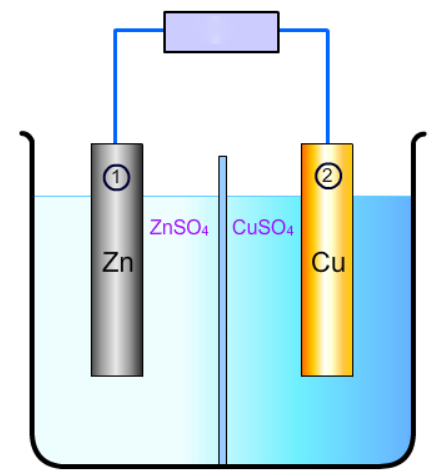
\includegraphics[width=.64\linewidth]{figures/zinc.png}
        \end{figure}
    \end{minipage}
    
\end{frame}


\begin{frame}
    \frametitle{金属-溶液界面电势差}

    金属晶格中有金属原子、金属离子和能够自由移动的电子存在。当金属浸在水中，极性很大的水分子可与金属表面的离子相互作用，水化的金属离子有可能离开金属表面进入水相，导致金属带负电荷，金属离子的水溶液带正电荷。

    \begin{minipage}{0.23\linewidth}
        \begin{figure}
            \centering
            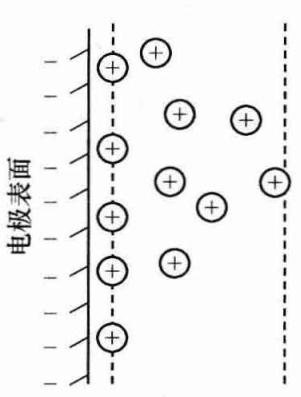
\includegraphics[width=\linewidth]{figures/fig6.2a.png}
        \end{figure}
    \end{minipage}\hfill
    \begin{minipage}{0.65\linewidth}
        \begin{itemize}
            \item[紧密层] 由于静电作用，水溶液相中金属离子聚集在界面附近，并可能沉积到金属表面，同时阻碍金属相的离子继续进入溶液，在界面附近形成一个电荷密度较大的紧密层。
            \item[扩散层] 由于溶液中离子的热运动和扩散作用，形成一个厚度稍大、电荷密度越来越小的扩散层。
        \end{itemize}
    \end{minipage}

    双电层是在金属-溶液界面上产生电势差的主要原因，该电势差称为电极的绝对电势，用\magenta{$\varepsilon$}表示。

\end{frame}


\begin{frame}
    \frametitle{液接电势}

        液体接界电势发生在两种电解质溶液的接界处。
        
        当两种不同电解质的溶液或电解质相同而浓度不同的溶液相接界时，由于电解质离子相互扩散时迁移速率不同，引起正、负离子在相界面两侧分布不均，导致在两种电解质溶液的接界处产生一微小电势差，称之为液体接界电势，也叫扩散电势，用\magenta{$\varepsilon _\text{扩散}$}表示。

    \begin{minipage}{0.48\linewidth}
        \begin{figure}
            \centering
            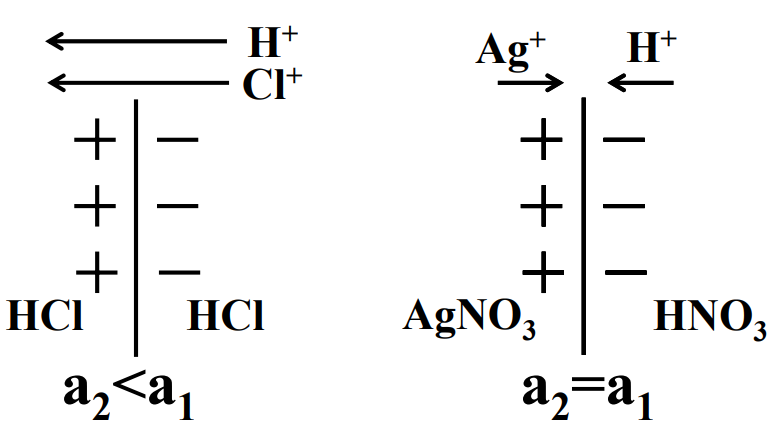
\includegraphics[width=\linewidth]{figures/fig6.2b.png}
        \end{figure}
    \end{minipage}\hfill
    \begin{minipage}{0.48\linewidth}
        常采用插入盐桥的办法尽量避免或减小液接电势。
        \begin{itemize}
            \item 盐桥中电解质的正、负离子的迁移速率几乎相等
            \item 盐桥两端产生的电势差方向相反，相互抵消
        \end{itemize}
    \end{minipage}

\end{frame}


\begin{frame}
    \frametitle{接触电势}

    在两种不同金属接界处，由于两种不同金属中的电子在接界处互相穿越的能力有差别，造成电子在界面两边的分布不均，缺少电子的一面带正电，电子过剩的一面带负电。当达到动态平衡后，在接触界面上就形成双电层，产生了电势差，称为接触电势。

    \begin{minipage}{0.34\linewidth}
        \begin{figure}
            \centering
            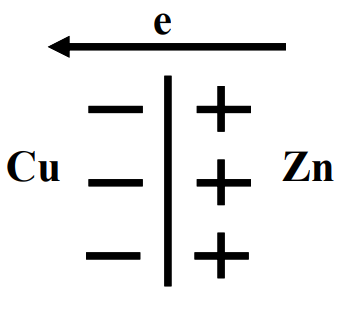
\includegraphics[width=\linewidth]{figures/fig6.2c.png}
        \end{figure}
    \end{minipage}\hfill
    \begin{minipage}{0.62\linewidth}
        原电池的两个电极常常是不同的金属，外电路用导线（通常是金属铜丝）与两极相连，因而产生接触电势。其大小与金属的本性有关，数值一般比较小，实验测定时可以忽略不计。
    \end{minipage}

\end{frame}


\begin{frame}
    \frametitle{电池的电动势}

    铜锌原电池可以表示为
    \[
        \mathrm{Cu}\text{(导线)}\ch{\ |\ Zn (s) \ |\  ZnSO4 ($b_1$)\ |\ CuSO4 ($b_2$)\ |\ Cu (s)}
    \]
    \[
        \quad \varepsilon_{\mathrm{Cu/Zn}} \quad \varepsilon_- \quad \qquad \varepsilon_{\text{扩散}}  \quad \qquad \varepsilon_+
    \]
    \[
        E = \varepsilon_{\mathrm{Cu/Zn}} + \varepsilon_- + \varepsilon_{\text{扩散}} + \varepsilon_+
    \]
    式中，$\varepsilon_{\mathrm{Cu/Zn}}$为接触电势，可忽略不计；
    
    $\varepsilon_{\text{扩散}}$可用盐桥消除；

    $\varepsilon_+$和$\varepsilon_-$分别为两电极的界面电势差，其绝对值无法求得。

    电池的电动势等于两电极绝对电势的代数和：
    \[
        E = \varepsilon_- + \varepsilon_+
    \]

\end{frame}


\begin{frame}
    \frametitle{电池的电动势}

    \large 两个标准电极组成的电池，则电池的标准电动势为
    \[
        E^{\ominus} = \varphi_+^{\ominus} - \varphi_-^{\ominus}
    \]
    一般将待测电极与任一已知电极电势的电极组成电池，根据电池电动势可得待测电极的电极电势。
    \[
        E^{\ominus} = \varphi_+ - \varphi_-
    \]
    可逆电池电动势$E$总是组成电池的两电极电势之差。

\end{frame}



\begin{frame}
    \frametitle{标准氢电极}

    一般用标准氢电极作标准以测定其他电极的相对电极电势数值。

    \begin{minipage}{0.58\linewidth}
        \[
            \mathrm{Pt (s),H_2}(p^\ominus)\ |\ \mathrm{H}^+(a_{\mathrm{H}^+}=1)
        \]
        \[
            \frac{1}{2}\mathrm{H_2}(p^\ominus) \longrightarrow \mathrm{H}^+(a_{\mathrm{H}^+}=1) + \mathrm{e}^-
        \]
        \[
            a_{\mathrm{H}^+}=1(b_{\mathrm{H}^+}=\SI{0.1}{mol.kg^{-1}})
        \]
        电化学规定，在指定温度下标准氢电极的电极电势$\varphi_{H_2}^\ominus=0 $
    \end{minipage}\hfill
    \begin{minipage}{0.35\linewidth}
        \begin{figure}
            \centering
            
\includegraphics[width=\linewidth]{figures/fig6.3.png}
            \caption{氢电极}
        \end{figure}
    \end{minipage}
\end{frame}


\begin{frame}
    \frametitle{电极电势$\varphi$}

    将标准氢电极作负极，给定的电极作正极组成电池：
    \[
        \mathrm{Pt (s),H_2}(p^\ominus)|\mathrm{H}^+(a_{\mathrm{H}^+}=1)||\text{给定电极}
    \]
    规定该电池电动势的数值和符号就是给定电极电势的数值和符号。
    \begin{itemize}
        \item 如给定电极实际上进行的反应是还原反应，则电极电势为正值；
        \item 如给定电极实际上进行的反应是氧化反应，则电极电势为负值。
    \end{itemize}
    \begin{example}
        \[
        \mathrm{Pt (s),H_2}(p^\ominus)|\mathrm{H}^+(a_{\mathrm{H}^+}=1)||\mathrm{Zn}^{2+}(a_{\mathrm{Zn}^{2+}}=1)|\mathrm{Zn(s)}
        \]
    \end{example}

\end{frame}


\begin{frame}
    \frametitle{}

    \begin{example}
        \[
        \mathrm{Pt (s),H_2}(p^\ominus)|\mathrm{H}^+(a_{\mathrm{H}^+}=1)||\mathrm{Zn}^{2+}(a_{\mathrm{Zn}^{2+}}=1)|\mathrm{Zn(s)}
        \]
        将锌电极与标准氢电极组成电池，实验测得电动势为\SI{0.7628}{V}。求$\varphi_{\mathrm{Zn^{2+}/Zn}}$。

        负极，阳极，氧化：
    \[
        \mathrm{H_2}(p^\ominus) \longrightarrow 2\mathrm{H}^+(a_{\mathrm{H}^+}=1) + 2\mathrm{e}^-
    \]
    正极，阴极，还原：
    \[
        \mathrm{Zn^{2+}}(a_{\mathrm{Zn^{2+}}}=1) + 2\mathrm{e}^- \longrightarrow \mathrm{Zn(s)}
    \]
    电池总反应：
    \[
        \mathrm{H_2}(p^\ominus) + \mathrm{Zn^{2+}}(a_{\mathrm{Zn^{2+}}}=1) \longrightarrow 2\mathrm{H}^+(a_{\mathrm{H}^+}=1) + \mathrm{Zn(s)}
    \]
    实际电池反应是上式的逆反应，所以为$\varphi$负值，即$\varphi_{\mathrm{Zn^{2+}/Zn}}=\SI{-0.7628}{V}$
    \end{example}
    
    
\end{frame}


\begin{frame}
    \frametitle{能斯特公式}

    \large 对于任意给定的一个电极，其电极还原反应写成如下通式：
    \[
        \text{氧化态} + n\mathrm{e^-} \longrightarrow \text{还原态} \quad \text{或} \quad \mathrm{Ox} + n\mathrm{e^-} \longrightarrow \mathrm{Red}
    \]
    则电极电势的通式为
    \[
        \varphi=\varphi^{\ominus}-\frac{R T}{n F} \ln \frac{a_{\mathrm{Red}}}{a_{\mathrm{Ox}}}=\varphi^{\ominus}+\frac{R T}{n F} \ln \frac{a_{\mathrm{Ox}}}{a_{\text {Red }}}
    \]
    上式即为能斯特(Nernst)公式。
    式中，$\varphi^{\ominus}$为标准状态下电极反应中各物质的活度均为1时的电极电势，称为该电极的标准电极电势。

    对整个电池反应：
    \[
        aA + dD +ne^- \rightarrow gG + hH
    \]
    \[
        \varphi=\varphi^{\ominus}-\frac{R T}{n F} \ln \prod \limits_{B} a_\mathrm{B}^{\nu_\mathrm{B}}
    \]
\end{frame}


\begin{frame}[t]
    \frametitle{}
    利用附录中的标准电极电势数据，可以计算一个可逆电池的标准电池电动势$E^{\ominus}$和电池电动势$E$。
    \begin{question}
        计算电池\ch{Zn (s) \ |\  Zn^{2+} (a = 0.1) \ ||\  Cu^{2+} (a = 0.1) \ |\  Cu (s)}的电动势。
    \end{question}
\end{frame}



\section{可逆电池热力学}


\begin{frame}
    \frametitle{电化学与热力学的联系}

    根据吉布斯自由能的定义知，在定温定压条件下，若电池可逆放电，体系吉布斯自由能的减少等于体系所做的最大非体积功。
    \[
        (\Delta_\mathrm{r}G_\mathrm{m})_{T,p} = W_\mathrm{max}^{'}
    \]
    可逆电功等于电动势与在该电动势作用下通过电量的乘积$qE$
    \[
        W_\mathrm{max}^{'} = -qE = -nFE
    \]
    所以
    \[
        \magenta{(\Delta_\mathrm{r}G_\mathrm{m})_{T,p} = -nFE}
    \]
    若电池两极的各种反应物质均处于标准状态，则
    \[
        \magenta{\Delta_\mathrm{r}G_\mathrm{m}^\ominus = -nFE^\ominus}
    \]

\end{frame}


\begin{frame}
    \frametitle{可逆电池电动势与活度和平衡常数}
    \[
        \ch{aA + dD == gG + hH}
    \]
    根据化学反应定温式，
    \[
        \Delta_{\mathrm{r}} G_{\mathrm{m}}=\Delta_{\mathrm{r}} G_{\mathrm{m}}^{\ominus}+R T \ln \frac{a_{\mathrm{G}}^{g} a_{\mathrm{H}}^{h}}{a_{\mathrm{A}}^{a} a_{\mathrm{D}}^{d}}
    \]
    \[
        -n F E=-n F E^{\ominus}+R T \ln \frac{a_{\mathrm{G}}^{g} a_{\mathrm{H}}^{h}}{a_{\mathrm{A}}^{a} a_{\mathrm{D}}^{d}}
    \]
    \[
        E=E^{\ominus}-\frac{R T}{n F} \ln \frac{a_{\mathrm{G}}^{g} a_{\mathrm{H}}^{h}}{a_{\mathrm{A}}^{a} a_{\mathrm{D}}^{d}}
    \]
    \[
        E^{\ominus}=\frac{R T}{n F} \ln K^{\ominus}
    \]

\end{frame}


\begin{frame}[t]
    \frametitle{}

    \begin{example}
        某电池反应可用如下两个方程表示，分别写出其对应的$\Delta_\mathrm{r}G_\mathrm{m}$，$K^{\ominus}$和$E$的表示式，并找出两组物理量之间的关系。

        (1) \ch{Zn(s) + Cu^{2+} (a_1) -> Zn^{2+} (a_2) + Cu (s)}

        (2) \ch{1/2 Zn(s) + 1/2 Cu^{2+} (a_1) -> 1/2 Zn^{2+} (a_2) + 1/2 Cu (s)}
    \end{example}

\end{frame}


\begin{frame}
    \frametitle{电动势与各热力学量}

    由吉布斯-亥姆霍兹公式${\left[\frac{\partial\left(\frac{\Delta G}{T}\right)}{\partial T}\right]_{p}=\frac{-\Delta H}{T^{2}} \text { 及 }(\Delta_{\mathrm{r}} G_{\mathrm{m}})_{T, p}=-n F E}$可得
    \[
        \Delta_{\mathrm{r}} H_{\mathrm{m}}=-n F E+n F T\left(\frac{\partial E}{\partial T}\right)_{p}
    \]
    $\left(\frac{\partial E}{\partial T}\right)_{p}$为电动势随温度变化率，又称电池电动势的温度系数。可由实验测得。

    结合$\Delta H=\Delta G+T \Delta S$，可得
    \[
        \Delta_{\mathrm{r}} S_{\mathrm{m}}=n F\left(\frac{\partial E}{\partial T}\right)_{p} 
    \]
    可逆电池的热效应$Q_{\mathrm{R}}=T \Delta S$，即
    \[
        Q_{\mathrm{R}}=n F T\left(\frac{\partial E}{\partial T}\right)_{p}
    \]
    由电池温度系数的正、负可确定可逆电池工作时是吸热还是放热。$\left(\frac{\partial E}{\partial T}\right)_{p}>0$，吸热。

\end{frame}


\begin{frame}[t]
    \frametitle{}
    
    \begin{example}
        \[
        \mathrm{Cd}(\mathrm{Hg})+\mathrm{Hg}_{2} \mathrm{SO}_{4}(\mathrm{~s})+\frac{8}{3} \mathrm{H}_{2} \mathrm{O}(\mathrm{l}) \longrightarrow \mathrm{CdSO}_{4} \cdot \frac{8}{3} \mathrm{H}_{2} \mathrm{O}(\mathrm{s})+2 \mathrm{Hg}(\mathrm{l})
        \]
        298K时，$E=$\SI{1.01832}{V}，$\left(\frac{\partial E}{\partial T}\right)_{p}=\SI{-5.00e-5}{V.K^{-1}}$。求298K时该电池反应的$\Delta_\mathrm{r}G_\mathrm{m}$、$\Delta_\mathrm{r}S_\mathrm{m}$、$\Delta_\mathrm{r}H_\mathrm{m}$、$\Delta_\mathrm{r}U_\mathrm{m}$、$Q_\mathrm{R}$和$W_\mathrm{max}^{'}$。
    \end{example}

\end{frame}


\begin{frame}[t]
    \frametitle{}

    \begin{example}
        已知273K时韦斯顿标准电池
        \[
            \ch{Cd(Hg) + Hg2SO4 (s) + 8/3 H2O -> CdSO4 . 8/3 H2O (s) + 2 Hg(l)}
        \]
        电动势为\SI{1.0186}{V}，$\left(\frac{\partial E}{\partial T}\right)_p=$\SI{-4.16e-5}{V.K^{-1}}，计算293K时电池反应的$\Delta_\mathrm{r}G_\mathrm{m}$、$\Delta_\mathrm{r}S_\mathrm{m}$、$\Delta_\mathrm{r}H_\mathrm{m}$、$\Delta_\mathrm{r}U_\mathrm{m}$、$Q_\mathrm{R}$和$W_\mathrm{max}^{'}$。
    \end{example}

\end{frame}


\section{电池电动势的测定及应用}


\begin{frame}
    \frametitle{对消法测电动势}

    \large 原电池的电动势等于没有电流通过时两极间的电势差，所以电动势常用对消法进行测定，而不能用伏特计或万用电表直接测定。
    \begin{itemize}
        \item 如果有电流通过，电池中就有化学反应发生，溶液的浓度发生变化，电池电动势也要发生变化。
        \item 由于电池本身有内阻，有电流通过，就会产生内电势降，用伏特计所测得的只是外电路上的电势降。
    \end{itemize}
    对消法测定原电池电动势的原理是，在外电路上联一个与待测电池电动势大小相等而方向相反的电池，以对抗原电池的电动势。

\end{frame}


\begin{frame}
    \frametitle{对消法测电动势}

    \begin{figure}[htpb]
        \centering
        
\includegraphics[width=.7\linewidth]{对消法}
    \end{figure}

        \begin{enumerate}
            \item 接通K1，将触点调到$C'$处，调节可变电阻R至G中无电流通过。
            \item 固定可变电阻R，接通K2，调节触点使中无电流通过，触点在C处。
        \end{enumerate}
        \[
            \magenta{E_x = E_s \frac{AC}{AC'}}
        \]

\end{frame}


\begin{frame}
    \frametitle{电位差计}

    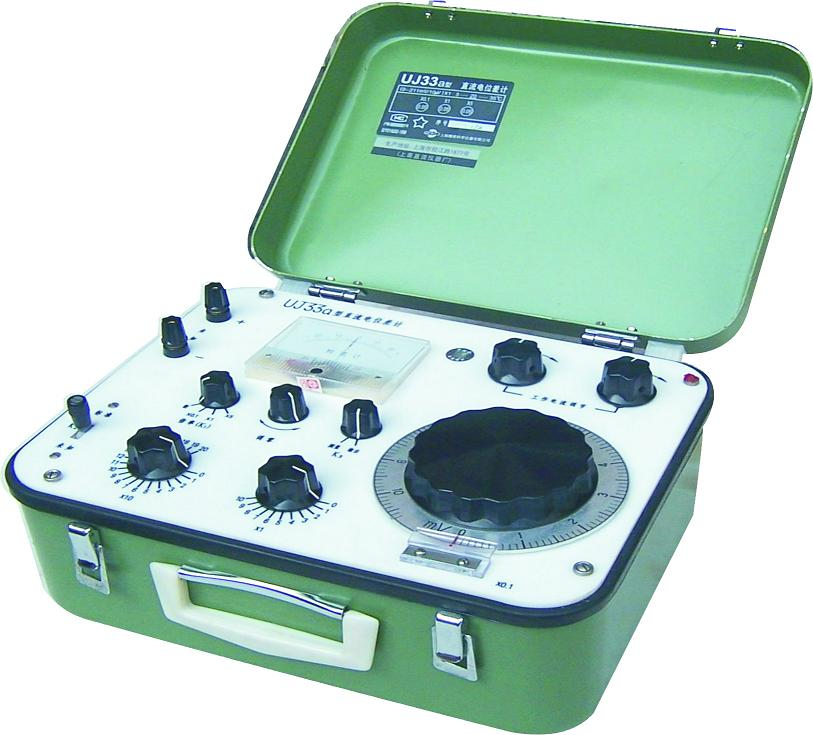
\includegraphics[width=.5\linewidth]{figures/R-C.jpg}

\end{frame}


\begin{frame}
    \frametitle{饱和韦斯顿标准电池}

    电位差计中所用的标准电池，其电动势必须精确已知，且能保持恒定。

    \begin{minipage}{0.3\linewidth}
        
\includegraphics[width=\linewidth]{figures/fig6.5.png}
    \end{minipage}\hfill
    \begin{minipage}{0.68\linewidth}
        \begin{itemize}
            \item 电池的充电、放电反应互为可逆
            \item 有很稳定的电动势
            \item 温度对其电池电动势影响很小
        \end{itemize}
        放电时：
        \[
            (-) \quad \ch{Cd(Hg) + SO4^{2-} + 8/3 H2O -> CdSO4 . 8/3 H2O (s) + 2 e-}
    \] 
        \[
            (+)\quad \ch{HgSO4(s) + 2 e- -> 2 Hg (l) + SO4^{2-}}
        \]
    \end{minipage}
    \[
            \text{总反应} \qquad \ch{Cd(Hg) + Hg2SO4 (s) + 8/3 H2O -> CdSO4 . 8/3 H2O (s) + 2 Hg(l)}
    \]

\end{frame}


\begin{frame}[t]
    \frametitle{电动势测定的应用}
    \begin{itemize}
        \item[1.] \cbf{化学反应平衡常数的测定}
    \end{itemize}
    根据实验测定或从标准电极电势数据计算出标准电池电动势值$E^\ominus$，就可以由式$E^\ominus = \frac{RT}{nF} \ln K^\ominus$计算出化学反应的平衡常数$K^\ominus$。
    \begin{example}
        试求反应\ch{2 Hg (l) + 2 Fe^{3+} (a_1) -> Hg2^{2+} (a_2) + 2 Fe^{2+} (a_3)}在298K时的标准平衡常数，已知$\varphi_{\ch{Hg2^{2+}/Hg}}^\ominus = 0.788V$，$\varphi_{\ch{Fe^{3+},Fe^{2+}/Pt}}^\ominus = 0.771V$。
    \end{example}

\end{frame}


\begin{frame}[t]
    \frametitle{电动势测定的应用}
    \begin{itemize}
        \item[2.] \cbf{难溶盐活度积常数$K_\mathrm{sp}$的测定}
    \end{itemize}
    将难溶盐溶解后形成离子的变化设计成电池，使电池反应就是难溶盐的溶解反应，根据标
准电极电势就可以求出$K_\mathrm{sp}$。
    \begin{example}
        298K时，$\varphi_{\ch{Ag^+/Ag}}^\ominus = 0.7991V$，$\varphi_{\ch{I^-,/AgI,Ag}}^\ominus = -0.152V$。求AgI的活度积$K_\mathrm{sp}$。      
    \end{example}\pause  
AgI的溶解反应为
        \[
            \ch{AgI (s) <=> Ag^+ (a_+) + I^- (a_-)}
        \]
        将此反应设计成电池
        \[
            \ch{Ag(s) \ |\  Ag^+ (a_+)\  ||\  I^- (a_-) \ |\  AgI (s),Ag (s)}
        \]
\end{frame}


\begin{frame}[t]
    \frametitle{电动势测定的应用}
    \begin{itemize}
        \item[3.] \cbf{离子平均活度系数的测定}
    \end{itemize}
    \begin{example}
        $$\begin{array}{c}
            {Pt}(\mathrm{s}), \mathrm{H}_{2}\left(p^{\ominus}\right)|\mathrm{HCl}(b)| \mathrm{AgCl}(\mathrm{s}), \mathrm{Ag}(\mathrm{s}) \\
            \frac{1}{2} \mathrm{H}_{2}\left(p^{\ominus}\right) \longrightarrow \mathrm{H}^{+}\left(a_{\mathrm{H}^{+}}\right)+\mathrm{e}^{-} \\
            \mathrm{AgCl}(\mathrm{s})+\mathrm{e}^{-} \longrightarrow \mathrm{Ag}(\mathrm{s})+\mathrm{Cl}^{-}\left(a_{\mathrm{Cl}^{-}}\right) \\
            \frac{1}{2} \mathrm{H}_{2}\left(p^{\ominus}\right)+\mathrm{AgCl}(\mathrm{s}) \longrightarrow \mathrm{Ag}(\mathrm{s})+\mathrm{H}^{+}\left(a_{\mathrm{H}^{+}}\right)+\mathrm{Cl}^{-}\left(a_{\mathrm{Cl}^{-}}\right)
        \end{array}$$
        $ \qquad
            E=E^{\ominus}-\frac{R T}{F} \ln (a_{\mathrm{H}^{+}} a_{\mathrm{Cl^-}})=E^{\ominus}-\frac{2 R T}{F} \ln a_{\pm}=E^{\ominus}-\frac{2 R T}{F} \ln \left(\gamma_{\pm} \frac{b_{\pm}}{b^{\ominus}}\right)
        $
        \[
            E+\frac{2 R T}{F} \ln \frac{b_{\pm}}{b^{\ominus}}=E^{\ominus}-\frac{2 R T}{F} \ln \gamma_{\pm}
        \]
        查表求得$E^{\ominus}$，测定某一浓度$b$时的电动势$E$，就可求出该浓度下的$\gamma_{\pm}$值。
            
    \end{example}

\end{frame}


\begin{frame}[t]
    \frametitle{电动势测定的应用}
    \begin{itemize}
        \item[4.] \cbf{pH的测定}
    \end{itemize}
    \begin{minipage}{0.32\linewidth}
        测定溶液的pH，可以用氢电极和一已知电极电势的参比电极组成电池。常用的参比电极是甘汞电极。氢电极是H$^+$指示电极，但由于制作和使用不方便，常用玻璃电极作H$^+$指示电极。
    \end{minipage}\hfill
    \begin{minipage}{0.65\linewidth}        
            
\includegraphics[width=\linewidth]{figures/fig6.6.png}        
    \end{minipage}
    
\end{frame}


\begin{frame}[t]
    \frametitle{电动势测定的应用}
    \begin{itemize}
        \item[4.] \cbf{pH的测定}
    \end{itemize}
    在用玻璃电极测定溶液pH时，将玻璃电极与甘汞电极组成的电池为
    \[
        \mathrm{Ag}(\mathrm{s}), \mathrm{AgCl}(\mathrm{s})|\mathrm{HCl}(0.1 \mathrm{~mol} \cdot \mathrm{kg}^{-1})| \mathrm{H}_{\text{(待测)}}^{+} \| \mathrm{KCl}  (\text{饱和})  \mid \mathrm{Hg}_{2} \mathrm{Cl}_{2}(\mathrm{s}), \mathrm{Hg}(\mathrm{l}) 
    \]
    298K时，
    \[
        E=\varphi_{\text {甘泵 }}-\varphi_{\text {玻 }}= \varphi_{\text {甘泵 }}-[\varphi_{\text {玻 }}^\ominus - \frac{2.303RT}{F}\mathrm{pH}] =0.2415 -(\varphi_{\text {玻 }}^{\ominus}-0.05916 \mathrm{pH})
    \]
    \[
        \mathrm{pH}=\frac{E-0.2415 \mathrm{~V}+\varphi_{\text {玻 }}^{\ominus}}{0.05916 \mathrm{~V}}
    \]
    测出电池电动势，已知$\varphi_{\text {玻 }}^\ominus$就可求出待测液的pH。

    对某给定玻璃电极$\varphi_{\text {玻 }}^\ominus$是一常数。


\end{frame}


\begin{frame}[t]
    \frametitle{电动势测定的应用}
    \begin{itemize}
        \item[4.] \cbf{pH的测定}
    \end{itemize}
    由于玻璃电极使用一段时间后表面状态会发生改变，在实际测量时，要先用已知pH的缓冲溶液对玻璃电极进行标定，在pH计上校准，然后在同样条件下测定未知液的pH，而不需求出的准确$\varphi_{\text{玻}}^{\ominus}$数值。

    298K时，未知液与标准缓冲溶液的$\mathrm{pH}_x$、$\mathrm{pH}_s$及电池电动势$E_x$、$E_s$之间关系
    \[
        \mathrm{pH}_x = \mathrm{pH}_s + \frac{E_x - E_s}{0.05916}
    \]
    \begin{example}
        298K时测定下列电池的电动势：玻璃电极|某种酸溶液||饱和甘汞电极。(1)$\mathrm{pH}=4.00$缓冲溶液，测得$E_1=\SI{0.1120}{V}$。换另一缓冲溶液，$E_2=\SI{0.2065}{V}$，求该缓冲溶液的pH。(2)若再换用$\mathrm{pH}=2.50$的缓冲溶液，$E$应为多少？
    \end{example}
    
\end{frame}



\begin{frame}[t]
    \frametitle{电动势测定的应用}
    \begin{itemize}
        \item[5.] \cbf{电势滴定}
    \end{itemize}
    电势滴定是根据电动势突变时加入滴定液的体积确定被分析离子活度的方法。

    \begin{minipage}{0.58\linewidth}
        \begin{itemize}
            \item 适用于指示剂难以监控滴定终点的反应
            \item 不需指示剂，操作简便
            \item 灵敏度高，准确度高
        \end{itemize}
    \end{minipage}\hfill
    \begin{minipage}{0.38\linewidth}        
            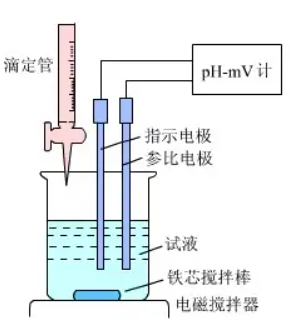
\includegraphics[width=0.75\linewidth]{figures/dianweididing.png}        
    \end{minipage}
    
    在滴定到达终点前后，滴液中的待测离子浓度往往连续变化n个数量级，因此电池电动势也会随之突变，根据电池电动势的突变指示滴定终点。

\end{frame}


\begin{frame}[t]
    \frametitle{电动势测定的应用}
    \begin{itemize}
        \item[6.] \cbf{离子选择性电极}
    \end{itemize}
    离子选择性电极是某离子的指示电极。常用的玻璃电极就是对H$^+$有选择性响应的指示电极。离子选择性电极具有离子感应膜，可以把溶液中某种离子的活度转换成相应的电势。测定方法是把离子选择性电极与参比电极（如甘汞电极）插入待测溶液组成电池，测定电动势，计算出离子的活度。

    例如，氟离子选择性电极
    \[
        \mathrm{AgCl}(\mathrm{s}), \mathrm{Ag}(\mathrm{s})\left|\begin{array}{l}
            \mathrm{F}^{-}(0.1 \mathrm{~mol} \cdot \mathrm{kg}^{-1}) \\
            \mathrm{Cl}^{-}(0.1 \mathrm{~mol} \cdot \mathrm{kg}^{-1})
            \end{array}\right| \mathrm{LaF}_{3} \mid \text { 含 } \mathrm{F}^{-} \text {的末知液 }
    \]        
    \[
        \varphi=\varphi^{\ominus}-\frac{2.303 R T}{F} \lg (a_{\mathrm{F}^{-}})_{\text {未知 }}
    \]

\end{frame}


\begin{frame}[t]
    \frametitle{电动势测定的应用}
    \begin{itemize}
        \item[7.] \cbf{浓差电池}
    \end{itemize}
    由两个组成相同但溶液中离子浓度不同或气体压力不同的电极构成的电池称为浓差电池。这种电池的标准电动势等于零。通过测定浓差电池的电动势可以测定电解质的活度、离子平均活度系数、离子迁移数等。
    \[
        \mathrm{Ag}(\mathrm{s}) \longrightarrow \mathrm{Ag}^{+}(a_{1})+\mathrm{e}^{-} \quad \varphi_{-}=\varphi^{\ominus}-\frac{R T}{F} \ln \frac{1}{a_{1}}
    \]
    \[
        \mathrm{Ag}^{+}(a_{2})+\mathrm{e}^{-} \longrightarrow \mathrm{Ag}(\mathrm{s}) \quad \varphi_{+}=\varphi^{\ominus}-\frac{R T}{F} \ln \frac{1}{a_{2}}
    \]
    \[
        \mathrm{Ag}^{+}(a_{2}) \longrightarrow \mathrm{Ag}^{+}(a_{1})
    \]
    \[
        E =\varphi_{+}-\varphi_{-}=\frac{R T}{F} \ln \frac{a_{2}}{a_{1}}
    \]
    

\end{frame}

\end{document}